\subsection{The ET cryostats}
In order to limit the thermal noise impact on the ET sensitivity curve it is necessary to cool at cryogenic temperature the four test masses of the LF-detector. The heat is extracted from the mirror via the suspension fibres attached at the other end to the marionette. Moreover, the marionette is suspended to the super-attenuator which attenuates the seismic noise up to few hertz. Thus, it is extremely important at the same time (i) to preserve the mechanical isolation between the mirror and the cooling system, (ii) to guarantee an efficient thermal link between the payload and the cooling system. 

% In figure%~\ref{fig:cryo_infrastructure_figure/ET_main-cryostat}
% we report a sketch of the cryo-mechanical system to be adopted for ET-LF. 
% \begin{figure}[t!] 
% \begin{center} 
% 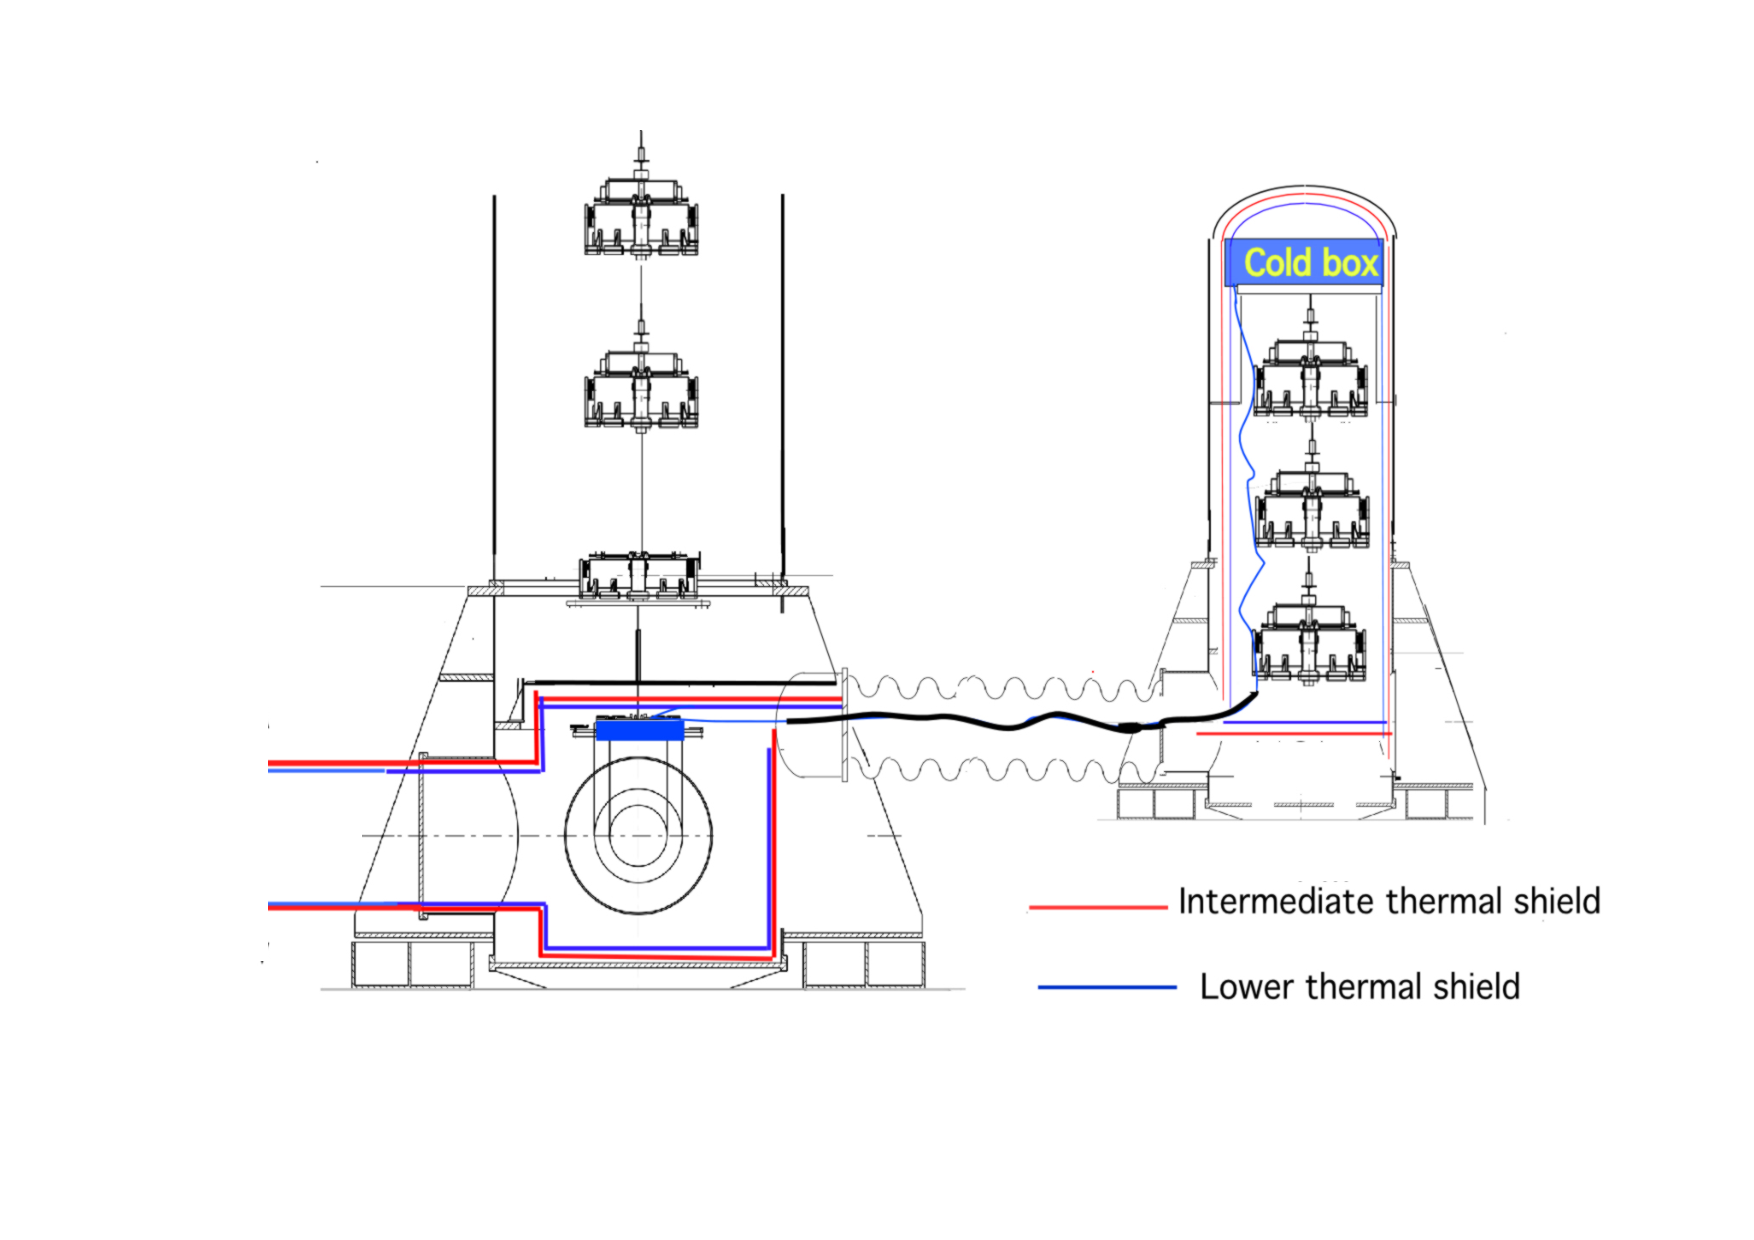
\includegraphics[width=17cm]{./Sec_SiteInfra/Figures/ET_main-cryostat.pdf} 
% \caption{Scheme of the cryostats needed for cooling a test-mass of the LF-interferometer.} \label{fig:cryo_infrastructure_figure/ET_main-cryostat}
% \end{center} 
% \end{figure} 

The whole payload is housed in the lower part of the vacuum tower hosting the 17-m long super-attenuator chain. The base of the vacuum tower is a cryostat with two thermal screens: the blue line schematizes a surface at $\sim4$\,K, while the red line represents the shield at intermediate temperature ($\sim 80$\,K). The upper part and lower part of the tower are separated by a roof crossed by the Ti-6Al-4V thin rod which holds the whole payload
%\footnote{The interface between the upper and lower suspension is described in section~(\ref{Upper_lower_suspension_interface}.}. 

The blue line defines a volume that has to be vacuum-tight. It will permit to cool-down and warm-up faster the whole payload by adding pure Helium gas in this experimental volume. Few mbars of helium will provide an efficient heat exchange during the cooling phase of the payload from room to cryogenic temperature. Once the equilibrium temperature is achieved, the helium gas is pumped out before the laser light injection. 

The base of the main tower hosting the mirror is connected to an ancillary tower shown in the figure. The ancillary tower  hoss the cold box, which will keep the mirror at cryogenic temperature. 
%The cold box can be either a simple liquid helium container in the case of a cryoplant based on cryofluids or the cold head of a cryo-refrigerator in the case of a cryocooler plant. 
A thermal line of $\sim 20$ m length connects the cold box to the last stage of the mirror suspension. It can be made of a braid of a high purity material as the electrolytic copper or the grade 6 aluminum (99.9999 \% purity). Both of them are metals characterized by thermal conductivity value of 2 kW/m/K in the range 1-10 K. In fact a braid of 20 m length, made of 8 wires 1 mm diameter can support an heat flow of 200 mW for a temperature difference of$\sim$ 1K at the link ends. To damp the vibration associated to the cooling system, the soft braid is mechanically coupled to the auxiliary super attenuator chain, hosted in the ancillary tower and fully complaint with the cryogenic environment. In order to define the requirement of the cryo plant we have to estimate the cryostat thermal inputs, which depend on the cryostat dimension and the quality of the thermal insulation. \noindent Assuming that the inner vacuum chamber has to host a mirror with a half meter diameter, we derived the order of magnitude of the thermal input for the cylindrical cryostats whose dimensions are reported in the following table: 
\begin{table}[htp] 
\caption{Cryostat dimensions} 
\begin{center} 
\begin{tabular}{|c|c|c|} \hline \hline Container & Diameter [m] & Height [m]\\ \hline Payload vacuum chamber & 1.5 & 3 \\ Auxiliary tower & 1 & 2 \\ \hline \hline
\end{tabular} 
\end{center} 
\label{tab:cryostat_dimension} 
\end{table} 

The thermal super insulation is a standard technique used in the modern cryostats. The thermal shield is formed by highly heat reflective thin layers, set under vacuum for increasing radiation reflection and decreasing radiation heat transfer through the insulation. The most known implementation is based on layers of porous (self-vented) mylar sheets, which are aluminized on one side. The sheets are wrapped around the surface to be insulated and form a multilayer blanket. The mylar is an hydroscopic material incompatible with the HUV requirements of ET. As a consequence the proposed solution implies to separate the chamber hosting the mirror to the insulation vacuum of the cryostat. A dedicated pumping system ( rotary-roots-turbo-molecular group) will provide the vacuum insulation. Wrapping 25 and 75 layers of self vented aluminized mylar around the two thermal shield, we achieve the condition to limit the thermal input below 1\,W for the 4\,K shields and around 50\,W for the intermediate ones. We assume in this evaluation that the thermal input due to laser light absorbed by the mirror and the thermal radiation emitted by the the km tube is in the range of few tens of milliwatts thanks to low silicon absorption at the laser wavelength and to the helium cryotraps described in~\ref{subsection_helium_cryotraps}. It is forth-worth to evaluate in more details these data in the context of the ET technical design study. 

\subsection{The LF-interferometer cryotraps}

\subsection{The cryogenic fluid distribution plant}
Cryogenic fluids in the form of liquid helium and liquid nitrogen are required to circulate for cooling the cryostats of the test masses and the associated cryotraps. The heat load requirement at a particular temperature is a prime important factor to select a helium refrigerator/liquefier and to define the dimensions of the nitrogen plant. The cryogenic systems of ET should operate in different modes cool down, steady state and warm up for each test mass tower, The cooling time is a trade off between the need to limit the detector down time and the stress due to the thermal gradients During cool down the recommended flow rate of helium gas will be approximately $\sim 1$\,g/s. The heat load requirement of cryogenic systems including the transfer loss at steady state is approximately $\sim 20$\,W at 4\,K helium refrigerator/liquefier. A helium refrigerator/liquefier having refrigeration capacity of 160\,W at 4\,K in refrigerator mode and 50\,L/h in liquefier mode without LN2 pre-cooling and 200\,W at 4.5\,K in refrigerator mode and 100\,L/h in liquefier mode with LN2 pre-cooling, is sufficient to guaranty the cooling in the vertex area of the triangular interferometer. In this evaluation a redundancy factor has been included so that the system will satisfactorily cater the refrigeration load at different state. As we anticipated before, to reach a full flexibility of the system, the possibility of performing the cool-down and the regeneration with the main refrigerator has been foreseen too. The cryogenic system will include a distribution valve box and the cryogenic piping up to the interface of the ET cryostat. The distribution valve box contains a 1000 L liquid helium control dewar, a heat exchanger, an electrical heater, a Joule-Thompson cryogenic valve and relevant instrumentation for pressure, temperature and flow rate measurements. The cryogenic system has to deliver, in a controlled way, the cooling helium from the refrigerators to the client. It includes mainly a 80\,K gas helium circuit and a 4.5\,K helium circuit, that can be interconnected through bypass valves; both shut-off valves and control valves are used. The 1000 L liquid helium dewar is used as buffer to stabilize the thermal loads and as re-cooler of the helium coming from the main refrigerator. An electrical heater and a cooling system are planned to make the system appropriate to operate an high temperature regeneration (470 K) and to cool it down again to room temperature. 
% \FloatBarrier \begin{figure}[htbp] \begin{center} \includegraphics[width=14cm, height=8cm]{./Sec_SiteInfra/Figures/He_plant_n.pdf} \caption{A simplified scheme of the cryogenic plant based on the use of cryofluids.} \label{fig:He_plant} \end{center} \end{figure} 

The redundancy of several elements is added to improve the reliability and the effectiveness of the cryoplant during the experimental conditions and to make it more flexible. The European industries have demonstrated there ability to construct complete refrigeration systems both for the needs of the huge accelerator and the associated detectors. Thus, the main refrigerators for ET will be realized with proven industrial technologies and tailored on the GW detector needs. It will be based on Claude cycle and it will provide the coolant helium at the required temperature for cooling the mirror. For the liquid helium distribution, we recall here that long and low thermal loss lines were developed at CERN already in the context of the LEP project. Since this time several improvements in design with respect to earlier lines of similar construction, made it possible to achieve reproducibly linear heat in-leaks of $\sim 30\,\mathrm{mW/m}$. At present the LHC refrigeration system is connected to the 27\,km long accelerator thanks to high performances helium transfer lines, which exhibit a variety of types, sizes, design choices and layouts. In the ET case the refrigerator will be installed on the surface building and the liquid helium has to be sent by long transfer lines to the underground detector, like the case of the LHC cryoplant. The transfer lines are based on the four-fold coaxial corrugated tube design Each line is made of austenitic stainless steel and the coaxial assembly provides an inner channel for the supply of liquid or gaseous helium an annular channel acting as a shield for the return of cold vapor, and a common vacuum enclosure for thermal insulation. Low thermal conductivity spacers, made of teflon PTFE are set between the outer tube, return channel and supply pipe. The outer corrugated tube of the return channel is also super-insulated by several layer of aluminized mylar (see figure~\ref{fig:transfer_line}). 
% \FloatBarrier \begin{figure}[htbp] \begin{center} 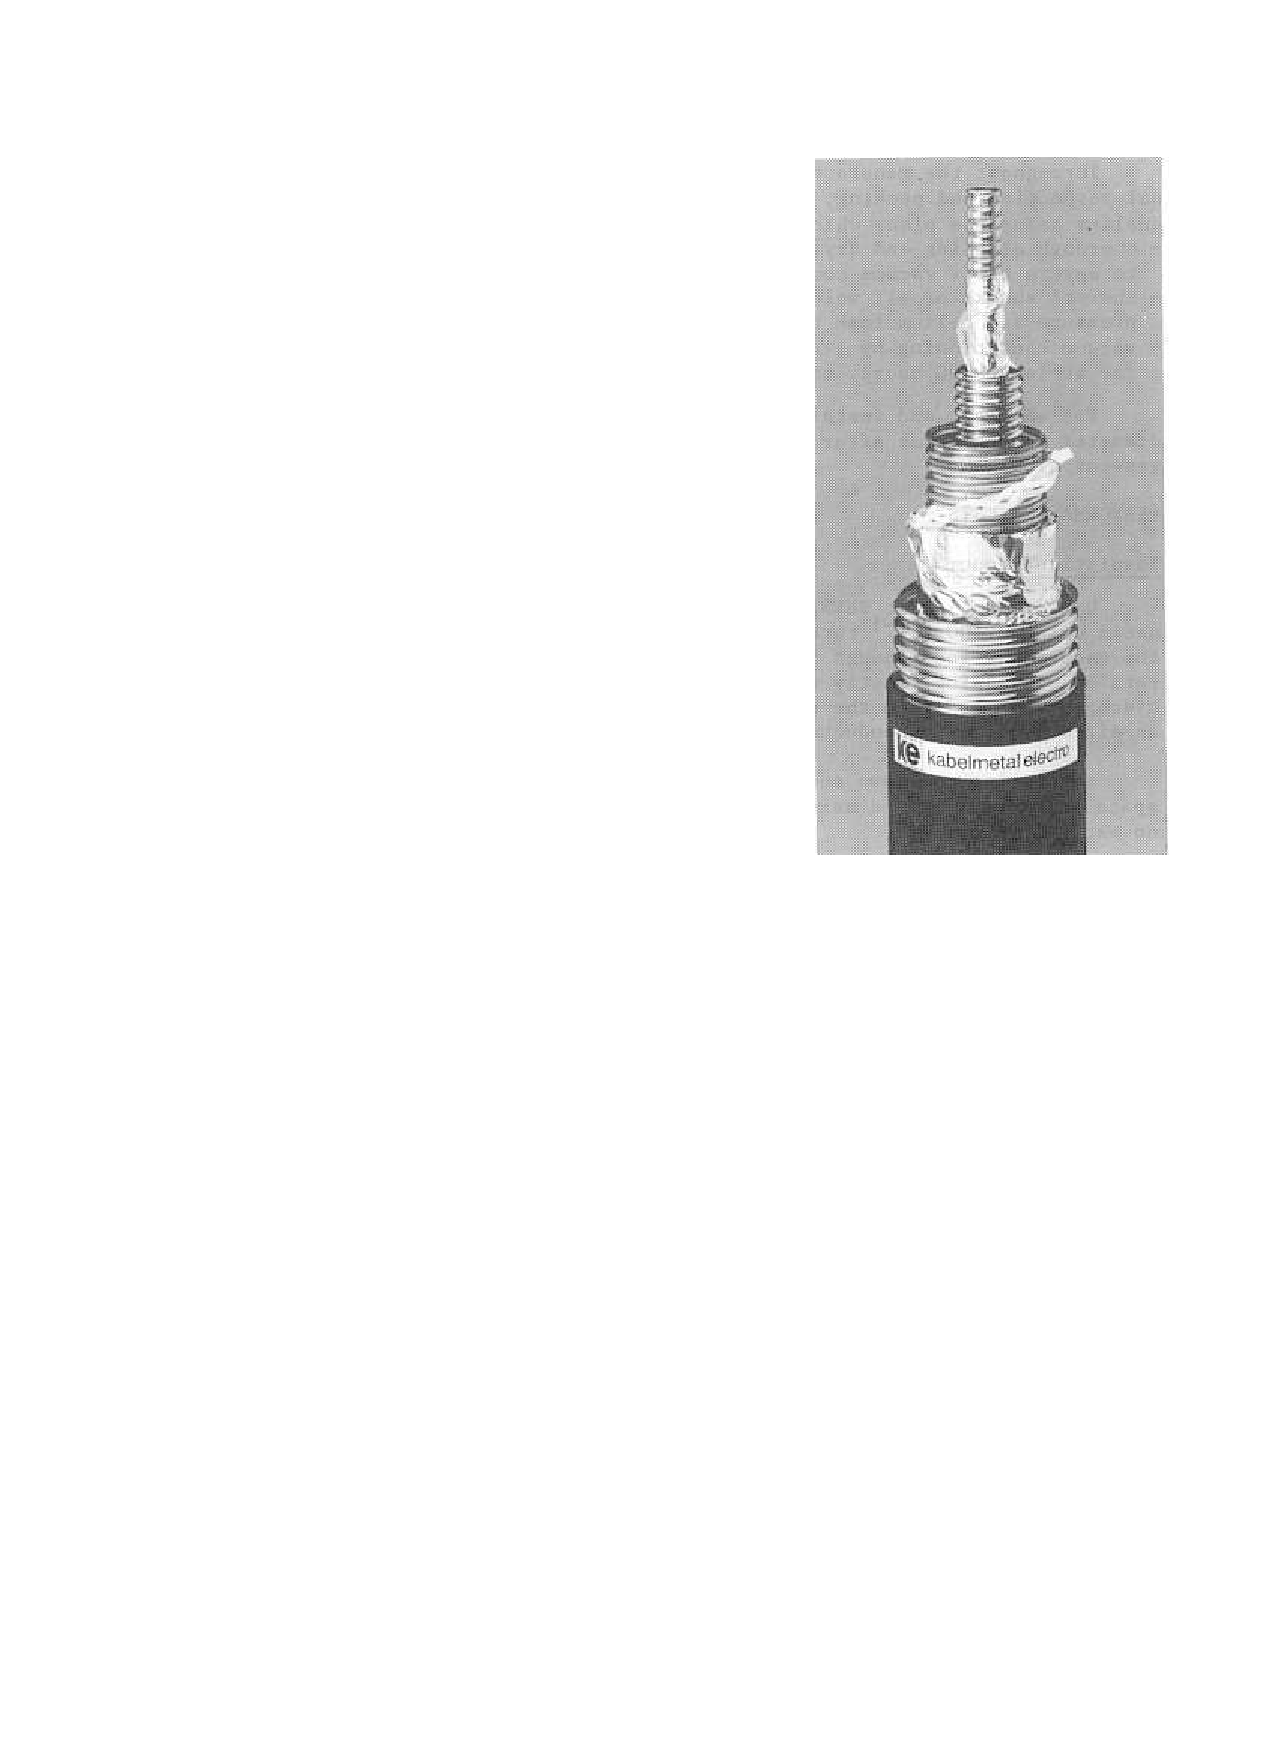
\includegraphics[width=5cm, height=7cm]{./Sec_SiteInfra/Figures/transfer_line.pdf} \caption{A cross section of a flexible transfer line developed at CERN in collaboration with Kabel Metalelectro~\cite{Lebrun}} \label{fig:transfer_line} \end{center} \end{figure} 

In order to reduce the quantity of impurities in the helium and to recover the gas, a Purification and Recovery System is implemented in the cryogenic plant. It is composed by a helium vaporizer, a high pressure recovery compressor and a helium cryogenic purifier system. An atmospheric gas bag (100 $m^3$), high pressure containers (20 bottles at 20 MPa, 10 N m$^3$ each) for impure gas helium, 3 medium pressure tanks (30 $m^3$ at 2 MPa) for pure gas helium, a liquid nitrogen container (50,000 L) and dedicated transfer stainless steel pipe lines are provided for the fluids storage. The helium to be recovered is collected in the gas bag; if its temperature is too low to enter in the gas bag, the cold helium is sent to a vaporizer where it is heated to the ambient temperature before entering the helium gas bag. The helium coming from the gas bag is sent to the recovery compressor and stored in the high pressure (20 MPa) bottles from which is delivered to the impure gas storage. The impure gas helium flows to the purifier and then it is stored in medium pressure (up to 2 MPa) pure helium buffers connected to the cycle compressors. The cryoplant will be installed in a building close to the main experiment building on surface. To reduce the noise trouble, due to the presence of compressors, a cryogenics compressor hall will be created as a separated part of the technical supplies building. The wall of this hall will be treated by a sound insulation system, to avoid noise transmission between the compressor hall and the other building. 

\subsubsection{Cryogenic plant control}
The cryoplant design and the technical solutions to be adopted are focused on the optimization of the system performances and it will be conceived to implement all the required operative scenarios in a fully automatic mode. 

The facility control system, based on a master/slave architecture, will be split into three plants (each for interferometer vertex ) and three distinct supervisory systems will be provided with engineer and operator workstations. The three control systems will be independent, but inter communication signals will be exchanged among the station units. The internal structure of the cryogenic control system will be based on PLCs (Programmable Logic Controllers), equipment of proven reliability in the industrial environment. A PLC will act as master of the local unit PLCs, with the purpose to coordinate the cryoplant activities and interface the logic unit with the upper subsystem level. Feedback control will be necessary to control for example the speed of the turbines or other parameters like temperature and pressure of the helium in different part of the cryogenic system; since the time constraints are not strict (response times of the order of seconds), the control routines will be executed without problems by PID (Proportional-Integral-Derivative) controllers inside the PLCs. A commercial off-the-shelf Supervisory Control and Data Acquisition system will be employed to monitor the plants, for operator intervention, commissioning, test purposes and data storage. 
